\documentclass{tpu-sotu}
\usepackage{ascmac}
\usepackage{cite}
\usepackage[dvipdfmx]{hyperref,graphicx}
\usepackage{pxjahyper}
\usepackage{listings,jlisting}
\lstset{language=C,%
    basicstyle={\ttfamily\small}, %書体の指定
    frame= tRBl, %フレームの指定
    framesep=10pt, %フレームと中身(コード)の間隔
    breaklines=ture, %行が長くなった場合の改行
    linewidth=12cm, %フレームの横幅
    lineskip=-0.5ex, %行間の調整
    tabsize=2 %Tabを何文字幅にするかの指定
	}%
%
% ここでタイトルの設定をします
%
% 自分の名前
\author{尾崎 裕樹}
%
% 学籍番号
\gakusekibangou{1515015}
%
% タイトル
\title{プログラミング演習における模範解答を用いた\\テストケース評価基準の自動生成}
\etitle{Automatic generation of evaluation criteria for test cases\\ using example codes in programming exercises}
%
% 日付
\date{2019年2月}
%
% 指導教員
\professor{中村 正樹 准教授}
%
% 所属
\department{電子・情報工学科}
%
%----- begin document
%
\begin{document}
%
\maketitle
\clearpage
\pagenumbering{roman}
\tableofcontents
\clearpage
\pagenumbering{arabic}
%

% - - - - - - - - - - - - - - - - - - -
%
\chapter{はじめに}
本研究では,プログラミング教育において,教員が学生の作成したプログラムに対して適切な評価を行う方法を考え,その際に利用できるシステムを提案する。
\section{背景}
プログラミング演習おいては,教科書のソースコードを書き写してプログラムを作成することから学習を始める学生もいる。教科書のコードが正確に書き写せているかの確認をするには,教科書のソースコードをと学生のソースコードを一字一句比較すればよい。
教科書のソースコードを書き写すだけではプログラムを作成できるようにはならないので,プログラミング演習では提示された仕様(課題や問題)を満たすプログラムを作成することを学ぶ必要がある。仕様を見てプログラムを作成した場合,一般に仕様を満たすプログラムは,一つに限らないため教員と学生が同じ実装をするとは限らず,教員の用意する模範解答のソースコードと学生のソースコードを単純に比較しただけでは正確な評価はできない。

通常,プログラムが仕様を満たすかどうかはソフトウェアテストにより確かめられる。
\begin{itemize}
\item ソフトウェアテスト
\begin{itemize}
\item ソフトウェアの品質を確保するためにプログラムが仕様通りに動作しているかを確認するために行う作業である。
\item ソフトウェアテストのテスト技法には,ホワイトボックステストとブラックボックステストがある。
\end{itemize}
\end{itemize}
\begin{itemize}
\item ホワイトボックステスト
\begin{itemize}
\item ソフトウェアの内部仕様やプログラムコードに基づいてテストケースを作成し,テストを実施する。
\end{itemize}
\end{itemize}
\begin{itemize}
\item ブラックボックステスト
\begin{itemize}
\item ソフトウェア内部の詳細を見ずに,プログラムに入力データを与え,実行結果だけを観測することで誤りを検出する。
\end{itemize}
\end{itemize}
\begin{itemize}
\item テストケース
\begin{itemize}
\item ソフトウェアテストを行うための入力と出力の組のことである。
\end{itemize}
\end{itemize}
教員がテストケースを用意する場合のプログラミング演習では,学生は用意されたテストケースでプログラムのテストを行うことで,プログラムが仕様を満たしているかを確認することができる。しかし,学生がテストケースを設計することを演習の対象とする場合も考えられる。
学生が設計したテストケースが適切であるか評価するには,ソースコードと同様に,教員のテストケースと学生のテストケースを一字一句の比較による評価では不十分である。
例えば,整数を入力して値が正の場合と負の場合,0の場合でそれぞれ異なる文字を表示するかをテストする場合を考える。学生と教員がテストケースの入力を表\ref{testcase}のように用意したとする。
\begin{table}[htb]
\centering
\caption{学生と教員のテストケース}
  \begin{tabular}{|c|c|c|} \hline
     & 学生 & 教員  \\ \hline
    テストケース1 & 1 & 2  \\ \hline
    テストケース2 & 0 & 0 \\ \hline
    テストケース3 & -4 & -3 \\ \hline
  \end{tabular}
  \label{testcase}
\end{table}
教員テストケースと学生のテストケースを比較すると正の場合と負の場合の入力が異なっているため,一字一句の比較では学生のテストケースは誤りと判断される。しかし,学生のテストケースでも3つの処理を確認することができるため,実際には誤りではない。したがって,学生の設計したテストケースが適切であるかを評価するための方法を考える必要がある。本研究におけるテストケース評価方法の位置づけを図\ref{a1}に示す。
\begin{figure}[h]
  \centering
  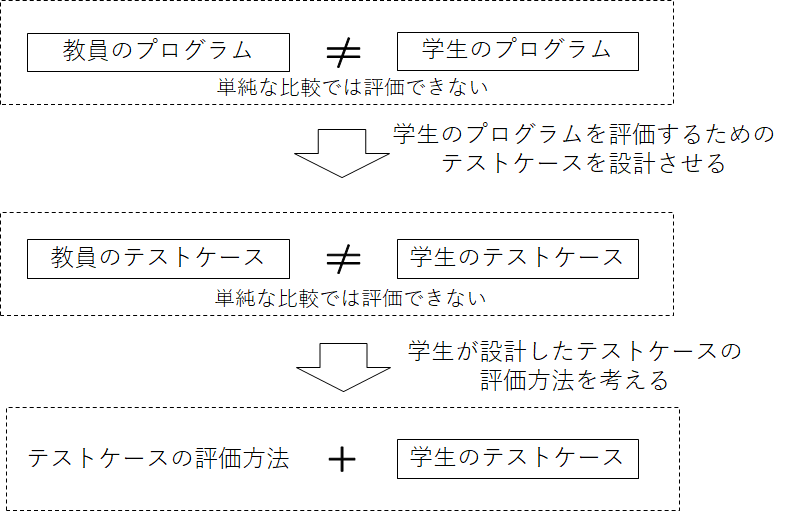
\includegraphics[width=130mm]{テストケース評価方法の位置づけ.png}
  \caption{テストケース評価方法の位置づけ}
  \label{a1}
\end{figure}
\newpage
テストケースを評価する方法の例として,文献~\cite{a0}では,テスト駆動開発に基づきプログラミング演習を行うことによってコーディングだけでなく,ソフトウェアテストの学習が行われる。評価対象は学生のプログラムとテストケースで,教員の作成したプログラムとテストケースを用いて図\ref{a2}のようにトリプルチェックテストを行うことによって評価される。
\newpage
\begin{figure}[h]
  \centering
  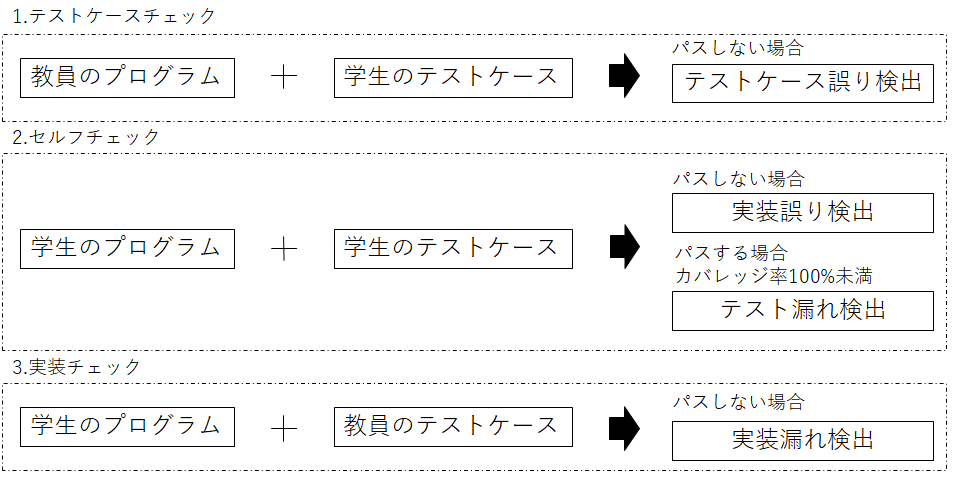
\includegraphics[width=130mm]{トリプルチェック.png}
  \caption{トリプルチェックテストによるコード判定原理}
  \label{a2}
\end{figure}

テストケースチェックによって,仕様要求を満たしていないテストケースが検出され,学生のテストケースの間違いが早期に指摘される。なお,仕様要求とは,プログラムにおける関数あるいはサブルーチンの動作が規定されたものであり,戻り値や引数などが定められたものである。教員のプログラムとテストケースはこの仕様要求が満たされるとする。
次のセルフチェックでは,テストの実行だけでなくコードカバレッジの測定が行われる。テストにパスしない場合は,学生のプログラムが正しく実装されていないことが分かり,テストにパスしたが,カバレッジが100\%でない場合は,テスト漏れが検出され学生に指摘される。最後の実装チェックでは,学生のプログラムが仕様要求の要求をすべて満たしていないことが検知され,次のテスト駆動開発サイクルを始めるよう学生に通知される。実装チェックをパスすることによって,学生が作成したプログラムとテストケースが仕様要求の要求をすべて満たしたことが確認される。

この手法では,テストケースの誤りを検出した際に,具体的にどのテストケースが不足しているのか学生に通知することができない。
そこで,テストケースが適切であるかを判定する評価基準を用意して,評価基準に対する設計したテストケースの網羅率を求めることで評価を行い,不足しているテストケースがあった場合にアドバイスを文献~\cite{a1}の手法の拡張を考える。
\section{目的}
本研究では,評価基準作成時における教員の負担を減らすために,テストケースの評価基準を自動化を行うことを目的とする。プログラムテストとテストケース評価基準,本研究で開発するシステムの関係を図\ref{a3}に示す。

\begin{figure}[h]
  \centering
  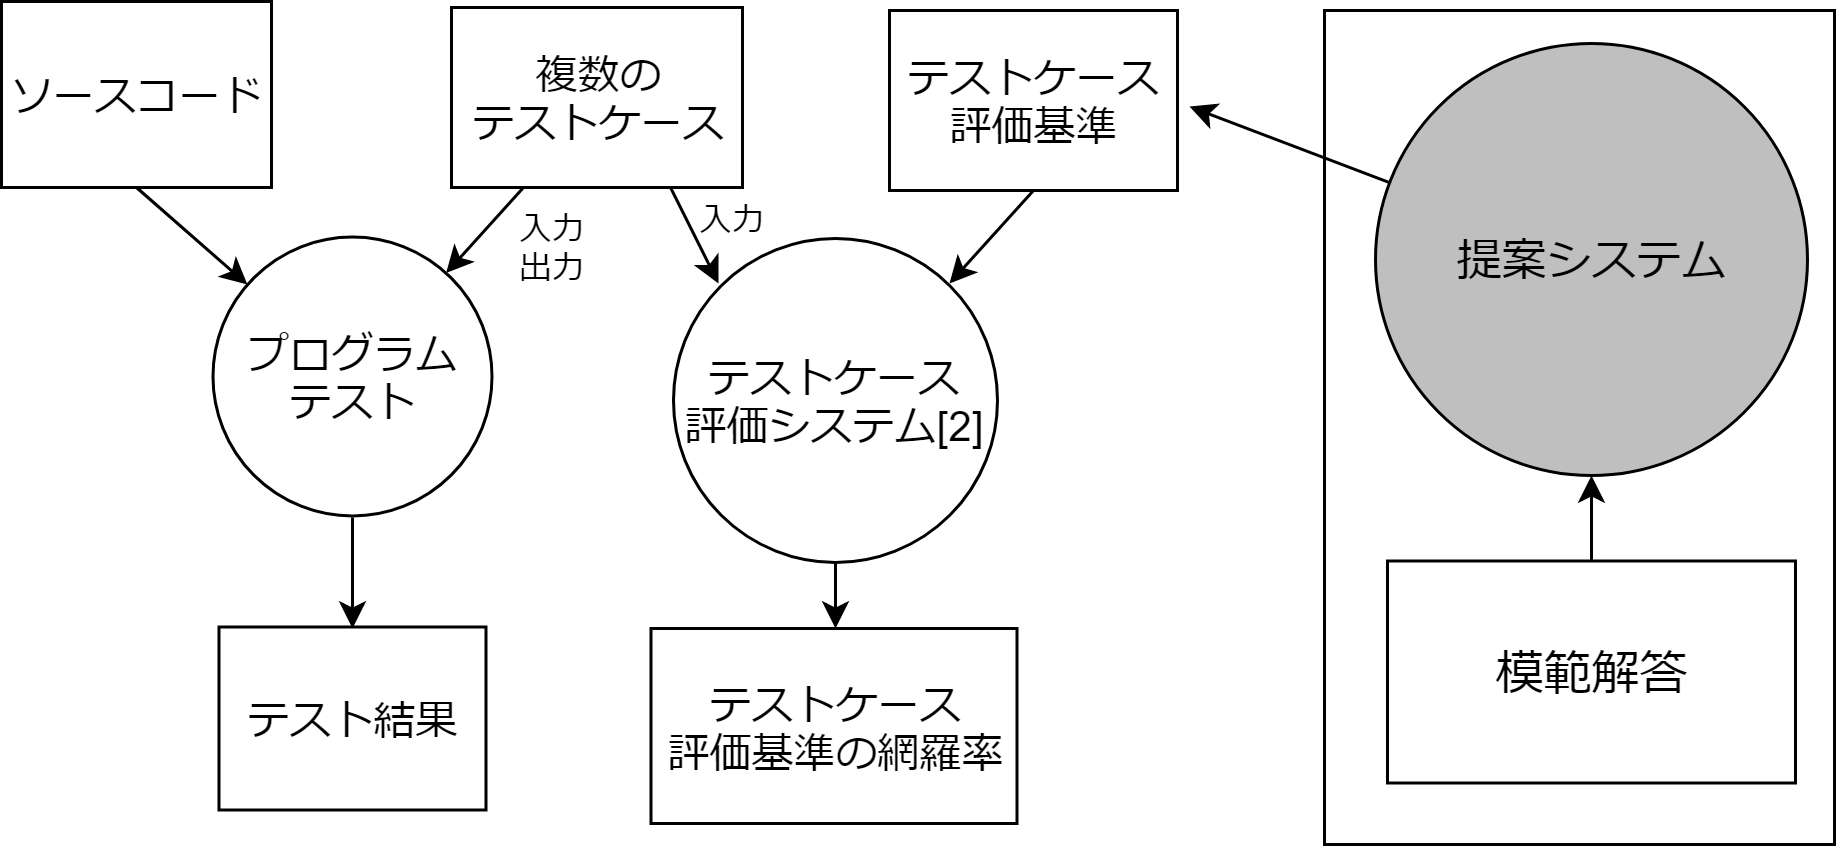
\includegraphics[width=130mm]{提案システムの位置づけ2.png}
  \caption{開発するシステムの位置づけ}
  \label{a3}
\end{figure}

\section{論文の構成}
以降,第2章では,関連研究としてテストケースの評価基準を用意してその網羅率によってテストケースを評価する手法を紹介する。第3章では,本研究で提案するテストケース評価基準の自動生成の手法についての説明および,評価基準生成システムを作成した手順について述べる。
\chapter{プログラミング演習におけるテストケース評価システム}
本章では文献~\cite{a1}で提案されているテストケース評価システムについて紹介する。テストケース評価システムでは,学生自身が適切なテストケースを設計できるようになるために,学生が作成したテストケースを評価してアドバイスを行うシステムが提案されている。このシステムでは,教員が演習問題毎にテストケースの評価基準とテストケースが不足していた場合に表示するアドバイスを与える必要がある。演習問題毎にテストしなければならない値や入力のデータ数が異なるため,評価基準は演習問題を分析した上で,入力のデータ構造を定義してから記述される。
\section{テストケース評価システム}
テストケース評価システムでは,教員があらかじめテストケース評価基準を作成し,学生が設計したテストケースが評価基準をどの程度パスできるかを判定することによって,テストケースの評価が行われる。評価基準をパスしない場合にアドバイスを表示することで,不足しているテストケースを学生に知らせる。テストケース評価システムにおいて,評価基準は次のようにタブ区切り形式でテキストとして記述される。\\
\begin{minipage}[b]{\textwidth}
\begin{itembox}[l]{評価基準の記述形式}
{\tt
 評価基準番号 TAB 判定条件 TAB アドバイス
}
\end{itembox}
\end{minipage}

「判定条件」はテストケースにおける入力データが満たすべき条件で,その条件を満たすテストケースがなかったときに,学習者に「アドバイス」が表示される。同値クラスを評価するための基準が複数ある場合などは,同じ「評価基準番号」を指定することで,評価基準がグループ化できる。例えば,年齢(整数値)を入力して,20歳以上は成年,20歳未満は未成年と表示する課題の評価基準は,入力データを変数ageとして,成年,未成年,エラーの場合について次のように記述される。\\
\begin{minipage}[b]{\textwidth}
\begin{itembox}[l]{評価基準の記述例1}
{\tt
1 TAB age==20 TAB 成年の最低年齢

1 TAB age>=20 TAB 成年の場合

2 TAB age==19 TAB 未成年の最高年齢

2 TAB age==0 TAB 0歳

2 TAB age>=0 \&\& age<20 TAB 未成年の場合

3 TAB age<0 TAB 年齢がマイナスの場合
}
\end{itembox}
\end{minipage}

学生が作成したテストケースの網羅率を,次の式で定義される評価基準のテストカバレッジにより提示する。\\
\begin{minipage}[b]{\textwidth}
\begin{itembox}[l]{評価基準のテストカバレッジ(%)}
{\tt
学習者のテストケースがパスした評価基準グループ数÷\\教員が記述した評価基準グループ数×100
}
\end{itembox}
\end{minipage}

判定条件の記述において,課題毎に入力データの型や個数が異なるため,テストケースの入力のデータ構造を定義し,そこで定義された変数を用いて判定条件が記述される。
\section{入力のデータ構造の定義}
データ構造は型と変数と出現回数から成る。入力のデータ構造の記述法はバッカス・ナウア記法(BNF)に類した形式で設計された。入力のデータ構造の定義例を以下に示す。なお,* は0回以上の繰り返しを表し,pintは正の整数,uintは0と正の整数,udoubleは0と正の実数の型である。\\
\begin{minipage}[b]{\textwidth}
\begin{itembox}[l]{データ構造の定義例}
(A)データ数(n)を入力し,その個数分身体データを入力する場合
{\tt

(pint n)

(pint id, string name, uint age, udouble height, udouble weight)\{n\}
}

(B)ファイルの終端まで分身体データを入力する場合
{\tt

(pint id, string name, uint age, udouble height, udouble weight)\{*\}
}

\end{itembox}
\end{minipage}

\section{関数定義}
判定条件の記述に関数を用いることができる。複数の身体データを読み込んで,身長の最大値を表示する課題の場合,最大値が複数存在するテストの評価基準は,引数のリストの最大値の個数を返す関数countmax()を定義して,次のように記述される。なお,実引数heightは全身長データのリストである。関数を評価基準で用いる場合,教員は関数定義も与える必要がある。\\
\begin{minipage}[b]{\textwidth}
\begin{itembox}[l]{関数を用いた評価基準の記述例}
{\tt
1 TAB countmax(height)>=2 TAB 身長の最大値が複数の場合
}
\end{itembox}
\end{minipage}
\begin{minipage}[b]{\textwidth}
\begin{itembox}[l]{countmax 関数}
{\tt
function countmax(\$list)\{

	\$lmax = max(\$list);

	return count(array\_keys(\$list, \$lmax));

\}
}
\end{itembox}
\end{minipage}

\section{評価基準の具体例}
入力が比較的複雑になる課題として,ボウリングの得点計算が例示されている。
\begin{itembox}[l]{ボウリングの点の計算の課題}
ボウリングは,1フレーム目から10フレーム目までの倒れたピンの数によって得点が決まる。フレームごとに倒したピンの数を読み込み,各フレームごとの得点を計算して表示すること。なお,ガーターとミスは0と表示するものとし,ダブルがあった場合はメッセージを表示する。
\end{itembox}
\begin{minipage}[b]{\textwidth}
\begin{itembox}[l]{ボウリングのデータ構造}
{\tt
(uint thr1, uint thr2)\{9\}

(uint last1, uint last2, uint last3)
}
\end{itembox}
\end{minipage}
\begin{itembox}[l]{ボウリングの評価基準}
{\tt
1 TAB thr1 == 10 TAB ストライクのスコア計算

2 TAB thr1 != 10 \&\& thr1+thr2 == 10 TAB スペアのスコア計算

3 TAB last1 == 10 TAB ストライクの通常加算

3 TAB last1 != 10  \&\& last1+last2 == 10 TAB スペアの通常加算

4 TAB double\_strike(thr1) || all\_strike([last1, last2]) TAB ダブル

4 TAB last\_strike(thr1) == 1 \&\& last1 == 10 TAB 最終Fをまたぐダブル
}
\end{itembox}

ストライクとスペアだった場合のスコア計算が正しいかをテストする必要がある(評価基準番号1, 2)。最終フレームではストライク,スペアでも通常の加算になるので,それらのテストも必要である(評価基準番号3)。評価基準番号4はダブルについてのテストである。ダブルがあればtrueを返す関数double\_strike(), リストがすべて10ならばtrueを返す関数all\_strike(),リストの最後の要素から10が何回連続しているかを返す関数last\_strike()が定義されている。
\section{システムの評価}
参考書の例題のテストケースのデータ構造が評価システムに則した形式で記述できるか調査が行われ,実行時に入力のデータ構造が変化する共用体などの問題以外ではデータ構造を記述できることが確認された。

また,評価システムにより,学生がテストケースを作成できるようになるのか確認をするために,プログラミングを学習済みの学生7人が評価システムを使ってボウリングの課題のテストケースを作成した。その結果最終的に6人の学生がカバレッジ100\%を達成したことが確認された。

\section{システムの課題}
テストケース評価システムでは,教員が問題文を分析した上で,評価基準を記述しているので,システムを運用する上で教員の負担が大きくなってしまうことが考えられる。

\chapter{テストケース評価基準の自動生成}
本章では,テストケース評価基準を自動で生成する手法の概要とシステムを作成する手順を示す。参考書~\cite{b1}に記述されている見本のプログラムを参考に評価基準生成システムを作成する。

\section{手法の概要}
前章のテストケース評価システムでは,教員が問題文を分析をし,テストケース評価基準や入力のデータ構造などを事前に記述しなければならない。そこで,プログラミング演習では,通常のソフトウェア開発と異なり教員が模範解答を用意しているという点に着目し,提案システムでは,テストケース評価基準を生成する際に,問題文(仕様)を分析して記述するのではなく,模範解答(ソースプログラム)を解析し,入力変数と条件式を抽出することによって,テストケース評価基準を生成する。また,入力された変数が正,負,0である場合のテストケースがあるのかを確認するためのテストケース評価基準を生成する。さらに,main関数以外の関数と関数の呼び出し部分を抽出し,テストケース評価基準とともに生成する。

\section{入力データの型に基づく評価基準}
まず,変数宣言から変数の型{\it t}と変数名{\it x}を抽出し保持する。標準入力命令\\
\[ 
\mbox{{\tt {scanf({\it f}, \&{\it x})}}}
\]
が現れた場合に,変数{\it x}の型を参照し,入力のデータ構造\\
\[
(t\:x)
\]
を生成する。変数{\it x}の型{\it t}が{\tt int, double, float}のいずれかであった場合は\\
\[ 
\mbox{\tt{{\it x} > 0}} 
\]
\[
\mbox{\tt{{\it x} == 0}}
\]
\[
\mbox{\tt{{\it x} < 0}}
\]
を評価基準として記述する。

以下に記述する入力された小数を表示するプログラムを用いて定義した通りの実相がされているかを確認する。
\lstinputlisting[xleftmargin=1cm]{source/Sample3_6.c}
このプログラムでは,変数宣言部分から{\tt double num}を取得し,標準入力命令\\
\[ 
\mbox{{\tt {scanf("\%lf", \&num)}}}
\]
から{\tt num}が入力変数であることを判定し,入力のデータ構造\\
\[
\mbox{{\tt double num}}
\]
が生成される。また,変数{\tt num}は{\tt double}型なので,変数{\tt num}の判別式\\
\[ 
\mbox{\tt{num > 0}} 
\]
\[
\mbox{\tt{num == 0}}
\]
\[
\mbox{\tt{num < 0}}
\]
がテストケース評価基準として生成される。
上記プログラムを入力としてシステムを実行した結果を以下に示す。
\lstinputlisting[xleftmargin=1cm]{result/resultS3_6.txt}
生成したテストケース評価基準をすべて満たすテストケースを入力とした場合の上記プログラムの実行結果を以下に示す。
\begin{lstlisting}[xleftmargin=1cm]
小数を入力してください。
1.2
1.200000が入力されました。
小数を入力してください。
0
0.000000が入力されました。
小数を入力してください。
-0.6
-0.600000が入力されました。
\end{lstlisting}

\section{条件文に基づく評価基準}
次に,条件判断文\\
{\tt \centerline {if({条件式})}}
が現れた場合に条件式を抽出することでテストケース評価基準を生成する。その際,分岐網羅をするために,条件文の否定もテストケース評価基準に含めて生成する。

以下に記述する入力された整数が1の場合とそれ以外の場合で異なる文字を表示するプログラムを用いて定義した通りの実相がされているかを確認する。
\lstinputlisting[xleftmargin=1cm]{source/Sample5_3.c}
このプログラムでは,変数宣言部分から{\tt int res}を取得し,標準入力命令\\
\[ 
\mbox{{\tt {scanf("\%d", \&res)}}}
\]
から{\tt res}が入力変数であることを判定し,入力データの構造\\
\[
\mbox{{\tt  int res}}
\]
が生成される。また,変数{\tt res}は{\tt int}型なので,変数{\tt res}の判別式\\
\[ 
\mbox{\tt{res > 0}} 
\]
\[
\mbox{\tt{res == 0}}
\]
\[
\mbox{\tt{res < 0}}
\]
がテストケース評価基準として生成される。また,条件判断文{\tt if}から条件式\\
\[
\mbox{\tt{res == 1}}
\]
とその否定\\
\[
\mbox{\tt{!(res == 1)}}
\]
がテストケース評価基準として生成される。
上記プログラムを入力としてシステムを実行した結果を以下に示す。
\lstinputlisting[xleftmargin=1cm]{result/resultS5_3.txt}
生成したテストケース評価基準をすべて満たすテストケースを入力とした場合の上記プログラムの実行結果を以下に示す。
\begin{lstlisting}[xleftmargin=1cm]
整数を入力してください。
1
1が入力されました。
整数を入力してください。
0
1以外が入力されました。
整数を入力してください。
-1
1以外が入力されました。
\end{lstlisting}

\section{関数を含むプログラムに対する評価基準}
さらに,関数宣言部から関数名を取得し,条件式で関数が使用されている場合は,評価基準とともに生成する。

以下に記述する入力された整数が偶数の場合と奇数の場合で異なる文字を表示するプログラムを用いて定義した通りの実相がされているかを確認する。
\lstinputlisting[xleftmargin=1cm]{source/odd.c}
このプログラムでは,変数宣言部分から{\tt int num}を取得し,標準入力命令\\
\[ 
\mbox{{\tt {scanf("\%d", \&num)}}}
\]
から{\tt num}が入力変数であることを判定し,入力データの構造\\
\[
\mbox{{\tt int num}}
\]
が生成される。また,変数{\tt num}は{\tt int}型なので,変数{\tt num}の判別式\\
\[ 
\mbox{\tt{num > 0}} 
\]
\[
\mbox{\tt{num == 0}}
\]
\[
\mbox{\tt{num < 0}}
\]
がテストケース評価基準として生成される。また,条件判断文{\tt if}から条件式\\
\[
\mbox{\tt{even(num) == 1}}
\]
とその否定\\
\[
\mbox{\tt{!(even(num) == 1)}}
\]
がテストケース評価基準として生成される。さらに,条件式に関数{\tt even()}が使用されているので,関数{\tt even()}の定義\\
\[ 
\mbox{\tt{int even(int num)    }} 
\]
\[
\mbox{\tt{\{             }}
\]
\[
\mbox{\tt{return num \% 2;}}
\]
\[
\mbox{\tt{\}             }}
\]
が生成される。
上記プログラムを入力としてシステムを実行した結果を以下に示す。
\lstinputlisting[xleftmargin=1cm]{result/odtest.txt}
生成したテストケース評価基準をすべて満たすテストケースを入力とした場合の上記プログラムの実行結果を以下に示す。
\begin{lstlisting}[xleftmargin=1cm]
整数を入力してください。
1
奇数です。
整数を入力してください。
0
偶数です。
整数を入力してください。
-3
奇数です。
整数を入力してください。

\end{lstlisting}
また,条件式に入力のない変数が使用されていて,その変数に関数を呼び出し,戻り値を代入している場合は,関数呼び出し部を生成する。

以下に記述する入力された整数が偶数の場合と奇数の場合で異なる文字を表示するプログラムを用いて定義した通りの実相がされているかを確認する。
\lstinputlisting[xleftmargin=1cm]{source/even.c}
このプログラムでは,変数宣言部分から{\tt int num}を取得し,標準入力命令\\
\[ 
\mbox{{\tt {scanf("\%d", \&num)}}}
\]
から{\tt num}が入力変数であることを判定し,入力データの構造\\
\[
\mbox{{\tt int num}}
\]
が生成される。また,変数{\tt num}は{\tt int}型なので,変数{\tt num}の判別式\\
\[ 
\mbox{\tt{num > 0}} 
\]
\[
\mbox{\tt{num == 0}}
\]
\[
\mbox{\tt{num < 0}}
\]
がテストケース評価基準として生成される。また,条件判断文{\tt if}から条件式\\
\[
\mbox{\tt{mod2 == 1}}
\]
とその否定\\
\[
\mbox{\tt{!(mod2 == 1)}}
\]
がテストケース評価基準として生成される。さらに,条件式に入力のない変数{\tt mod2}が使用されていて,{\tt mod2}に対して関数{\tt even()}を呼び出し,戻り値を代入しているので,関数{\tt even()}の定義\\
\[ 
\mbox{\tt{int even(int num)    }} 
\]
\[
\mbox{\tt{\{             }}
\]
\[
\mbox{\tt{return num \% 2;}}
\]
\[
\mbox{\tt{\}             }}
\]
と関数呼び出し部\\
\[
\mbox{\tt {mod2 = even(num)}}
\]
が生成される。上記プログラムを入力としてシステムを実行した結果を以下に示す。
\lstinputlisting[xleftmargin=1cm]{result/evtest.txt}
\chapter{プログラミング課題への適用}
この章では,参考書~\cite{b1}の練習問題の模範解答から評価基準が生成できるかを検証する。
参考書~\cite{b1}の5章(場合に応じた処理)までのサンプルコードや練習問題のうち,標準入力があるプログラムを対象に,作成したシステムによってテストケース評価基準の生成が可能か検証した。
検証を行ったプログラムは26個であり,そのうちの17個で生成可能であった。生成できなかったプログラムはgetcharで入力を行っているプログラムと,同じ変数に複数回入力しているプログラム,switch文や条件演算子で場合分けをしているプログラムであった。また,関数を含むプログラムに対して評価基準を生成できるか確認するために,身長と体重を入力しbmiを計算し,肥満度を表示するプログラムでも検証を行った。

\section{評価基準を生成できた問題}
\begin{itembox}[l]{問題1}
身長を入力した後に体重を入力して順番に表示する。
\end{itembox}
\lstinputlisting[xleftmargin=1cm]{source/3_4.c}
このプログラムでは,変数宣言部分から{\tt double height}と{\tt double weight}を取得し,標準入力命令\\
\[ 
\mbox{{\tt {scanf("\%lf", \&height)}}}
\]
\[ 
\mbox{{\tt {scanf("\%lf", \&weight)}}}
\]
から{\tt height}と{\tt weight}が入力変数であることを判定し,入力のデータ構造\\
\[
\mbox{{\tt double height}}
\]
\[
\mbox{{\tt double weight}}
\]
が生成される。また,変数{\tt height}と変数{\tt weight}は{\tt double}型なので,変数{\tt height}と変数{\tt weight}の判別式\\
\[ 
\mbox{\tt{height > 0}} 
\]
\[
\mbox{\tt{height == 0}}
\]
\[
\mbox{\tt{height < 0}}
\]
\[ 
\mbox{\tt{weight > 0}} 
\]
\[
\mbox{\tt{weight == 0}}
\]
\[
\mbox{\tt{weight < 0}}
\]
がテストケース評価基準として生成される。
\lstinputlisting[xleftmargin=1cm]{result/result3_4.txt}
\begin{lstlisting}[xleftmargin=1cm]
身長を入力してください。
160
体重を入力してください。
50
身長は160.000000センチです。
体重は50.000000キロです。
身長を入力してください。
0
体重を入力してください。
0
身長は0.000000センチです。
体重は0.000000キロです。
身長を入力してください。
-100
体重を入力してください。
-40
身長は-100.000000センチです。
体重は-40.000000キロです。
\end{lstlisting}
\begin{itembox}[l]{問題2}
キーボードから整数を2つ入力させ,値が大きいほうを表示する。
\end{itembox}

\lstinputlisting[xleftmargin=1cm]{source/5_2.c}
このプログラムでは,変数宣言部分から{\tt int num1}と{\tt int num2}を取得し,標準入力命令\\
\[ 
\mbox{{\tt {scanf("\%d", \&num1)}}}
\]
\[ 
\mbox{{\tt {scanf("\%d", \&num2)}}}
\]
から{\tt num1}と{\tt num2}が入力変数であることを判定し,入力のデータ構造\\
\[
\mbox{{\tt int num1}}
\]
\[
\mbox{{\tt int num2}}
\]
が生成される。また,変数{\tt num1}と変数{\tt num2}は{\tt int}型なので,変数{\tt num1}と変数{\tt num2}の判別式\\
\[ 
\mbox{\tt{num1 > 0}} 
\]
\[
\mbox{\tt{num1 == 0}}
\]
\[
\mbox{\tt{num1 < 0}}
\]
\[ 
\mbox{\tt{num2 > 0}} 
\]
\[
\mbox{\tt{num2 == 0}}
\]
\[
\mbox{\tt{num2 < 0}}
\]
がテストケース評価基準として生成される。また,条件判断文{\tt if}から条件式\\
\[
\mbox{\tt{num1 < num2}}
\]
\[
\mbox{\tt{num1 > num2}}
\]
とそれぞれの否定\\
\[
\mbox{\tt{!(num1 < num2)}}
\]
\[
\mbox{\tt{!(num1 > num2)}}
\]
がテストケース評価基準として生成される。
\lstinputlisting[xleftmargin=1cm]{result/result5_2.txt}
\begin{lstlisting}[xleftmargin=1cm]
整数を入力してください。
1
1は奇数です。
整数を入力してください。
0
0は偶数です。
整数を入力してください。
-2
-2は偶数です。
\end{lstlisting}
\lstinputlisting[xleftmargin=1cm]{source/bmi.c}
\lstinputlisting[xleftmargin=1cm]{result/bmiResult.txt}
\begin{lstlisting}[xleftmargin=1cm]
   ソースコード
\end{lstlisting}
\section{評価基準を生成できなかった問題}
\begin{itembox}[l]{問題3}
キーボードから5人分のテストの点数を入力させ,最高点を表示する。
\end{itembox}
\lstinputlisting[xleftmargin=1cm]{source/4_5.c}
このプログラムでは,変数{\tt num}に対して入力が三回行われているので入力のデータ構造として
\[
\mbox{{\tt (int num)}\{3\}}
\]
が生成されなければならないが,現在は同じ変数が複数回入力される場合に回数を表示させることができず,
\[
\mbox{{\tt (int num)}}
\]
のみ生成される。
\begin{itembox}[l]{問題4}
入力された整数が1ならAコース,それ以外ならBコースを表示する。
\end{itembox}
\lstinputlisting[xleftmargin=1cm]{source/Sample5_7.c}
このプログラムでは,変数{\tt res}が1か否かの判定が行われているため,条件式
\[
\mbox{\tt{res == 1}}
\]
\[
\mbox{\tt{!(res == 1)}}
\]
が生成されなければならないが,現在は条件判断文{\tt if}以外からは条件式を抽出できないため,条件文に基づく評価基準が生成できない。
\chapter{おわりに}
本研究では,学生が自身でテストケースの評価を行うために用いるテストケース評価基準を自動生成する方法を提案した。
現在対応できていない配列や繰り返し文,関数を含むプログラムからの評価基準の自動生成が今後の課題である。

\acknowledgements
本研究を進めていく中で,多くの助言とご指摘をいただきました中村正樹准教授,榊原一紀准教授に心より感謝の意を表します。また,合同ゼミにおいて,助言とご協力をいただきました中村研究室,榊原研究室の皆様に感謝いたします。
\begin{thebibliography}{2}
   \bibitem{a0} 吉田英輔,角川裕次: テスト駆動開発に基づくプログラミング学習支援システム : 初心者開発者のためのセルフトレーニングアーキテクチャ,信学技報.\\SS,ソフトウェアサイエンス,Vol.105,No.331(2005),pp.27-32
   \bibitem{a1} 蜂巣吉成,小林悟,吉田敦,阿草清磁: プログラミング演習におけるテストケース評価システム,コンピュータソフトウェア第34巻第4号,2017,pp.54-60
   \bibitem{b1} 高橋麻奈: やさしいC,SB クリエイティブ,2012
\end{thebibliography}

\end{document}
